\subsection{Diffusion models samplers}

Sampling from diffusion model can take thousands of denoising steps. In this section we will see common samplers used in the literature to sample from diffusion models for faster inference. But first we begin with the forward and reverse diffusion process as described in the DDPM paper \cite{ddpm}.








\subsubsection*{Forward process}

In the forward process we can take step-by-step approach (adding noise at each step, current step depends on previous step only):

\[ q(x_t | x_{t-1}) := \mathcal{N} \left( \sqrt{\frac{\alpha_t}{\alpha_{t-1}}} x_{t-1}, \left( 1 - \frac{\alpha_t}{\alpha_{t-1}} I \right) \right) \]

where $\alpha \in (0, 1]$ is the scaling factor of the noise scheduler, $\alpha_t$ is the noise added at timestep $t$.

However in the DDPM paper \cite{ddpm} they showed that we can go from $x_0$ (the original image without any noise added) to $x_T$ (pure Gaussian noise) in one step:

\[ q(x_T | x_0) := \mathcal{N} \left( x_t; \sqrt{\alpha_t} x_0, (1 - \alpha_t) I \right) \]

But because its not streightforward to implement, they used the \textbf{repametrization trick}:

\[ x_t = \sqrt{\alpha_t} x_0 + \sqrt{1 - \alpha_t} \epsilon \]

where $\epsilon \sim \mathcal{N} (0, I)$. 








\subsubsection*{Backward process}

The backward process is when we go from noisy image and denoise it to get the original image. The backward process is described as:

\[ p_\theta (x_{0:T}) := p(x_T) \prod_{t=1}^{T} p_\theta (x_{t-1} | x_t) \]

where $p(x_T)$ is the sampled noisy image (Gaussian noise) and we iteratively multiply by the denoising procesure where each step depends on the previous step.









\subsubsection{DDPM Sampler}

\begin{figure}
    \centering
    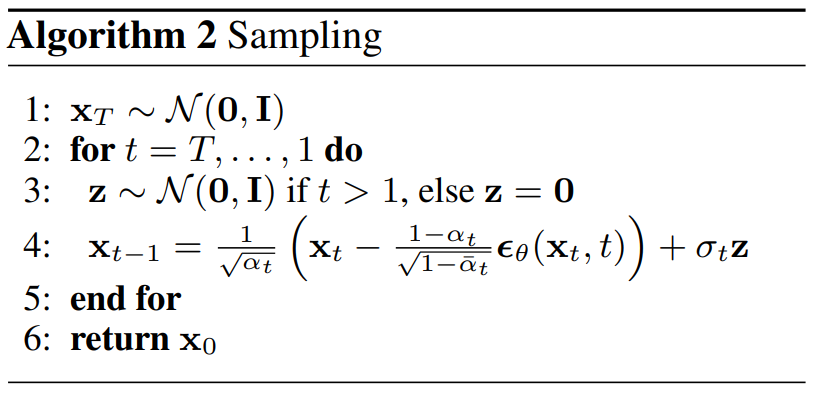
\includegraphics[width=0.5\textwidth]{images/appendix/dm_samplers/ddpm.png}
    \caption{DDPM sampler. Sampling process from the DDPM paper \cite{ddpm}.}
    \label{fig:appendix_ddpm_sampling}
\end{figure}

The denoising diffusion probabilistic model (DDPM) sampler is shown in figure \ref{fig:appendix_ddpm_sampling}. At first we sample random Gaussian noise $x_T \sim \mathcal{N} (0, I)$. Then for $T$ iterations we slowly denoise the image:

\[ x_{t-1} = \frac{1}{\sqrt{\alpha_t}} \left( x_t - \frac{1 - \alpha_t}{\sqrt{1 - \bar{\alpha_t}}} \epsilon_\theta (x_t, t) \right) + \sigma_t z \]

where $\epsilon_\theta$ is the denoising neural network (that predicts the noise) with the inputs $(x_t, t)$, and we remove that noise with $\left( x_t - \frac{1 - \alpha_t}{\sqrt{1 - \bar{\alpha_t}}} \right)$ where $\bar{\alpha}_t = \prod_{s=1}^{t} \alpha_s$. The last element: $\sigma_t z$ is to add variance to the generated samples. For instance, if $z=0$ then every time we generate an image from the same noisy image $x_T$ we get the same result (the same cat for instance). But if we add some variance to it, we get different cats every time we sample from the same noisy image $x_T$. When we reach $t=0$ then we set $z=0$ to get the final denoised image $x_0$ without variance.







\subsubsection{DDIM Sampler}

One problem of denoising an image is that there are multiple paths of the denoising steps to take; in two denoising steps, we can reach the same result but in different ways. For example, the first denoising step removes $x$ amount of noise and the second steps removes $y$ amount of noise, totaling $x+y$ noise removes; but we can also remove $y$ amount of noise at the first step and $x$ amount at the second step.

The denoising diffusion implicit models (DDIM) paper \cite{ddim} suggest non-markovian approach to fast infer samples from the diffusion model.







\subsubsection{SDE Sampler}

...